%% GR4AD — WSDM 2027 submission (ACM acmart, sigconf, double-blind review).
%% Requires acmart.cls (TeX Live `tlmgr install acmart`, or compile on Overleaf).
%% Title is a placeholder; all experimental numbers trace to experiments/*/results.json.
\documentclass[sigconf,anonymous,review]{acmart}

\AtBeginDocument{%
  \providecommand\BibTeX{{\normalfont B\kern-0.5em{\scshape i\kern-0.25em b}\kern-0.8em\TeX}}}
\settopmatter{printacmref=false}
\setcopyright{none}
\acmConference[WSDM '27]{The 20th ACM International Conference on Web Search and Data Mining}{February 2027}{Hong Kong}

\usepackage{booktabs}
\usepackage{graphicx}

\begin{document}

\title{Recalibrating Overconfident Generative Retrievers: A Model-Agnostic Post-hoc Reranking Scorer}

\author{Anonymous Authors}
\affiliation{%
  \institution{Submitted for double-blind review}
  \country{}
}

\begin{abstract}
Generative retrieval models decode item identifiers token-by-token and rank candidates by sequence
log-probability, but we show these scores are badly mis-calibrated: a frozen generator places most of
the catalog's relevant items inside its beam yet ranks them poorly---a \emph{confidence cascade} in
which per-position calibration error explodes along the decoded code while chain recall collapses.
Closing this gap is hard because the generator is expensive to retrain and its overconfidence is
intrinsic to autoregressive decoding. We introduce a lightweight \emph{post-hoc reranking scorer}
that leaves the generator frozen, rescoring its beam-50 candidates by fusing the beam log-probability
with a learned relevance score, $\mathrm{final}=\mathrm{avg\_logprob}+\lambda\cdot\mathrm{scorer}$,
where the fusion weight $\lambda$ is chosen per setting by an identical held-out validation
procedure. Across four settings spanning two base
architectures (a $k$-means semantic-ID generator and a T5 autoregressive decoder), two domains (news,
e-commerce), and three code-lengths (4/7/5), the \emph{same} method improves Recall@1 by 3.2--6.3\%
with the listwise variant, significant at Recall@10 in all four settings (5/5 seeds, McNemar
$p<10^{-6}$), and reduces per-candidate calibration error from 0.283 to 0.0009.
\end{abstract}

\keywords{generative retrieval, recommendation, reranking, calibration, semantic IDs}

\maketitle

\begin{figure}[t]
  \centering
  
\includegraphics[width=\linewidth]{figures/teaser.pdf}
  \caption{A frozen generative retriever emits an overconfident beam (high calibration error, low
  Scoring Efficiency): the target is usually \emph{in} the beam but ranked poorly. Our model-agnostic
  post-hoc scorer rescores the \emph{same} beam, fusing the generator's $\mathrm{avg\_logprob}$ with a
  calibrated relevance term ($\lambda$ chosen on held-out validation), recalibrating the scores and
  lifting Recall@1 by 3.2--6.3\% across diverse base generators---without retraining the generator.}
  \label{fig:teaser}
\end{figure}

\section{Introduction}
Generative retrieval has emerged as a compact alternative to dual-encoder retrieval: an
encoder--decoder model autoregressively generates a target item's discrete identifier (a sequence of
semantic or hierarchical codes), and beam search produces a ranked candidate
list~\cite{tiger,gram,idgenrec,lcrec,letter}. The model's own sequence log-probability serves as the
ranking score. This is elegant---one model both generates and ranks---but it couples \emph{recall}
(is the target in the beam?) to \emph{ranking} (is it near the top?) through a single signal the
decoder was never trained to calibrate (Fig.~\ref{fig:teaser}).

\paragraph{We first diagnose a confidence cascade.} On a frozen generator we measure, per decoded
position, the expected calibration error (ECE) of the decoder's token confidence. Under greedy
decoding ECE rises from 0.007 at the first position to 0.890 by the last, while the fraction of beams
whose entire code chain is consistent with the target collapses from 0.084 to 0.029. Crucially, the
target is \emph{recoverable}: Oracle Recall (target anywhere in the beam) far exceeds vanilla
Recall@1---the Scoring Efficiency $R@1/R@50$ is only 9--19\% across settings. The generator finds the
right items but ranks them with an overconfident, mis-calibrated score.

\paragraph{We then close the gap with a model-agnostic post-hoc scorer.} Rather than retrain the
(expensive, frozen) generator, we rerank its beam-50 candidates with a small scorer trained only on
validation beams. The reranked score fuses the generator's evidence with the learned relevance,
$\mathrm{final}=\mathrm{avg\_logprob}+\lambda\cdot\mathrm{scorer}$. The fusion weight $\lambda$ is the
single per-setting free parameter; we select it by an \emph{identical} procedure on a held-out split
of validation users that the scorer never trained on. Holding this selection \emph{procedure}---not a
fixed $\lambda$ value---constant across settings is what lets the method transfer.

\paragraph{Contributions.}
\begin{itemize}
\item We characterize a \textbf{confidence cascade} in generative retrievers: token-level
overconfidence compounds along the decoded code, so beam log-probability is a weak ranking signal
despite high beam recall (\S\ref{sec:cascade}, Fig.~\ref{fig:cascade}).
\item We propose a \textbf{model-agnostic post-hoc reranking scorer} (listwise and pointwise variants)
with a \textbf{held-out $\lambda$-selection} procedure, and show the procedure---not just the
architecture---is the control variable that makes the method transfer (\S\ref{sec:method}).
\item We validate model-agnosticism across \textbf{four settings} (2 base architectures $\times$ 2
domains $\times$ 3 code-lengths): listwise Recall@1 $+3.2$--$6.3\%$, Recall@10 significant in all four
(5/5 seeds, McNemar $p<10^{-6}$), and per-candidate ECE $0.283\to0.0009$ (\S\ref{sec:exp}).
\end{itemize}

\section{Related Work}
\paragraph{Generative retrieval / recommendation.} Generating item identifiers and ranking by
sequence likelihood~\cite{tiger,gram,idgenrec,lcrec,letter}. These works focus on \emph{building} the
generator (better identifiers, training objectives); we treat any such generator as frozen and address
the \emph{ranking} of its beam, which is complementary.
\paragraph{Calibration of neural models.} ECE, reliability diagrams, and temperature
scaling~\cite{guo_calibration}; we measure the per-candidate calibration of a generative retriever and
show a learned scorer recalibrates it.
\paragraph{Learning-to-rank objectives.} Pointwise focal loss~\cite{focal_loss}, listwise
likelihood (ListMLE)~\cite{listmle}, and smoothed-rank surrogates (ApproxNDCG)~\cite{approxndcg}; our
diagnostic finds binary BCE best for this rerank setting.
\paragraph{Discriminative baselines.} SASRec~\cite{sasrec} (sequential) and NRMS~\cite{nrms} (news),
compared under a matched full-catalog protocol.

\section{The Confidence Cascade}\label{sec:cascade}
On the frozen MIND generator we decode the 4-token code and, at each position, bin the decoder's
max-softmax confidence against token correctness to obtain per-position ECE, under both greedy and
oracle (teacher-forced) decoding. Greedy ECE $=[0.007,0.360,0.901,0.890]$ versus oracle
$[0.007,0.068,0.035,0.011]$: errors compound only when the model conditions on its own (overconfident)
predictions. Chain recall drops from 0.084 ($t_0$) to 0.029 (all four), yet Oracle $R@50$ (0.367)
$\gg$ $R@1$ (0.033). The ranking signal, not recall, is the bottleneck (Fig.~\ref{fig:cascade}).

\begin{figure}[t]
  \centering
  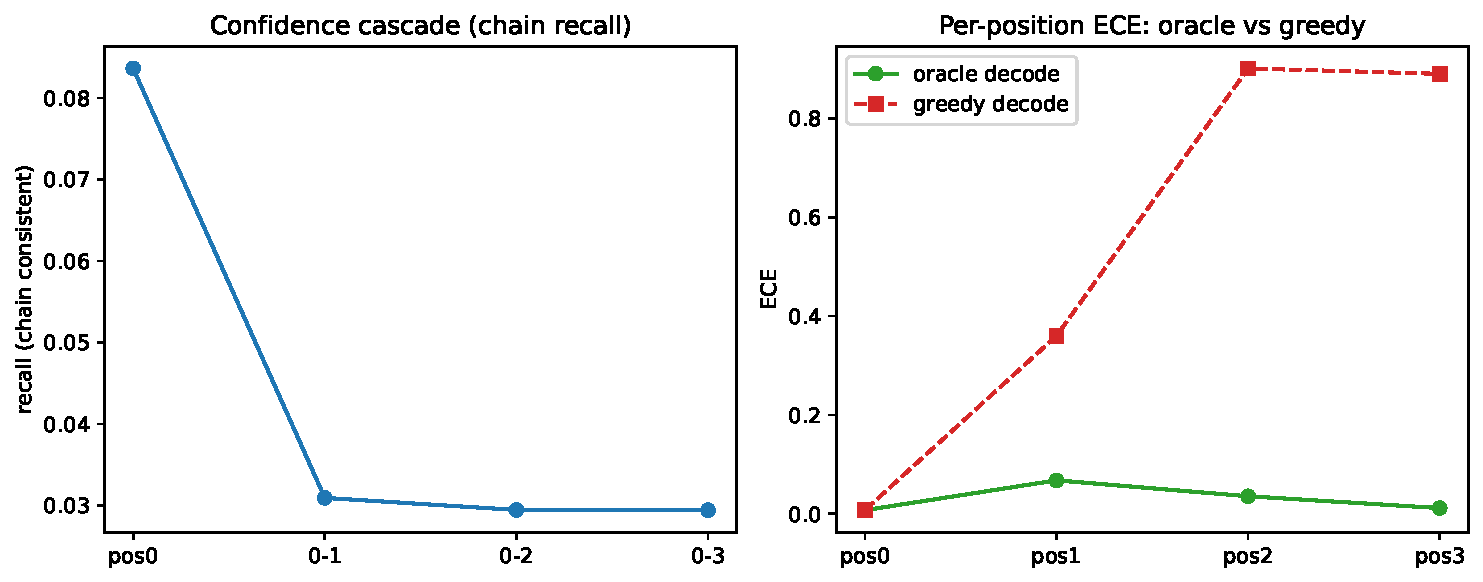
\includegraphics[width=\linewidth]{figures/confidence_cascade.pdf}
  \caption{Confidence cascade on the frozen MIND generator. Left: chain recall collapses as the
  decode chain extends (pos0$\to$pos3). Right: per-position ECE explodes under greedy decoding
  (0.890 at the last position) but stays low under oracle decoding (0.011), exposing the
  overconfidence the scorer must recalibrate.}
  \label{fig:cascade}
\end{figure}

\section{Method}\label{sec:method}
\paragraph{Setup.} A frozen generator produces, per query, a beam of $K{=}50$ candidate codes with
sequence log-probabilities. Let $s$ be the candidate's average token log-probability. A scorer $f$
maps the candidate's decoder hidden states (and the user representation) to a relevance term; we
rerank by $\mathrm{final}=s+\lambda\,f(\cdot)$. $\lambda{=}0$ recovers vanilla ranking; $\lambda{\to}\infty$
is scorer-only.

\paragraph{Scorer variants (held constant across all settings).}
\emph{Listwise}---self-attention over the beam ($d{=}128$, 4 heads, 2 layers, FFN 256, dropout 0.1, a
user-CLS token, and the beam score as a feature), trained with binary BCE. \emph{Pointwise Focal}---a
per-candidate MLP with a 64-d bottleneck, focal BCE ($\gamma{=}2.0$).

\paragraph{Held-out $\lambda$-selection (the control variable).} We split validation \emph{users} into
a pool (70\%, trains the scorer) and a disjoint holdout (30\%, selects $\lambda$). $\lambda$ is chosen
by argmax Recall@1 on the holdout over a fixed grid $\{0,0.02,0.05,0.1,0.2,0.35,0.5,0.7,1.0\}$; the
5-seed listwise uses one shared $\lambda$. The transfer claim rests on holding this
procedure---not a fixed $\lambda$ value---constant: the scorer method, hyperparameters, and
$\lambda$-selection procedure are byte-identical across settings (the control), while the base
generator (architecture, tokenizer, code-length, domain, eval split) is the treatment.

\section{Experiments}\label{sec:exp}
\paragraph{Settings.} (1) MIND-small news, a $k$-means semantic-ID generator, code-length 4, user
70/15/15 split; (2--4) Amazon Beauty/Sports/Toys, a T5 autoregressive decoder, code-length 7/7/5,
leave-one-out. Beam $K{=}50$ (per-sample), seeds $\{42,123,7,999,2024\}$.

\paragraph{Protocol.} All rows report Recall@$K$/MRR/nDCG@$K$ of their own ranked list via one shared
metric implementation. Generative rows (vanilla/Focal/Listwise/Oracle) are \emph{beam-recall-bounded}
(rank within the $K{=}50$ beam, so $R@50{=}$Oracle); the discriminative baselines NRMS/SASRec rank the
\emph{full catalog}. Absolute Recall@$K$ is therefore not directly comparable across the two families
(footnoted in each table); the within-family generative comparison (vanilla $\to$ scorer) is the
controlled test of our contribution.

\begin{table}[t]
  \caption{News (MIND-small, user-split, full-catalog). Generative rows are beam-bounded; NRMS ranks
  the full catalog (not directly comparable; see text). Listwise vs.\ vanilla: McNemar $R@1$
  $p{=}3.5{\times}10^{-4}$, $R@10$ $p{=}1.3{\times}10^{-6}$; 5/5 seeds significant. $^{**}p<0.01$.}
  \label{tab:news}
  \begin{tabular}{lccc}
    \toprule
    Method & R@1 & R@10 & R@50 \\
    \midrule
    NRMS (full-catalog) & 0.0015 & 0.0174 & 0.0610 \\
    Vanilla generator & 0.0331 & 0.1692 & 0.3671 \\
    \quad + Pointwise Focal & 0.0345\,(+4.1\%) & 0.1710 & --- \\
    \quad + Listwise (5-seed)$^{**}$ & \textbf{0.0352\,(+6.3\%)} & 0.1723 & --- \\
    Oracle & 0.3671 & 0.3671 & 0.3671 \\
    \bottomrule
  \end{tabular}
\end{table}

\begin{table}[t]
  \caption{E-commerce (Beauty/Sports/Toys, leave-one-out, full-catalog), Recall@10. Listwise $R@1$
  lift vs.\ vanilla: Beauty $+5.0\%$, Sports $+6.5\%$, Toys $+3.2\%$. Listwise vs.\ vanilla McNemar
  $R@10$: $p{=}2.1{\times}10^{-8}$/$2.2{\times}10^{-8}$/$2.7{\times}10^{-11}$, 5/5 seeds each.}
  \label{tab:ecom}
  \begin{tabular}{lccc}
    \toprule
    Method & Beauty & Sports & Toys \\
    \midrule
    SASRec (full-catalog) & 0.0133 & 0.0104 & 0.0112 \\
    Vanilla generator & 0.0881 & 0.0561 & 0.0927 \\
    \quad + Pointwise Focal & 0.0923 & 0.0601 & 0.0957 \\
    \quad + Listwise (5-seed) & \textbf{0.0944} & \textbf{0.0606} & \textbf{0.0979} \\
    Oracle & 0.1731 & 0.1207 & 0.1662 \\
    \bottomrule
  \end{tabular}
\end{table}

\paragraph{Main results.} Tables~\ref{tab:news} and~\ref{tab:ecom} show that one identical
held-out $\lambda$-selection procedure yields a positive, Recall@10-significant listwise lift in all four settings
(2 architectures $\times$ 2 domains $\times$ code-lengths 4/7/5). Recall@1 is significant on MIND
(user-split, multiple samples per user) but not under Amazon leave-one-out single-target sparsity, so
we report Recall@10/McNemar as primary for LOO.

\paragraph{Calibration.} On MIND, the generator's absolute confidence $\exp(\mathrm{avg\_logprob})$ is
badly overconfident (per-candidate ECE 0.283), while the listwise scorer's calibrated probability
achieves ECE 0.0009 (Fig.~\ref{fig:ece})---the scorer recalibrates the over-confident generator,
consistent with \S\ref{sec:cascade}.

\begin{figure}[t]
  \centering
  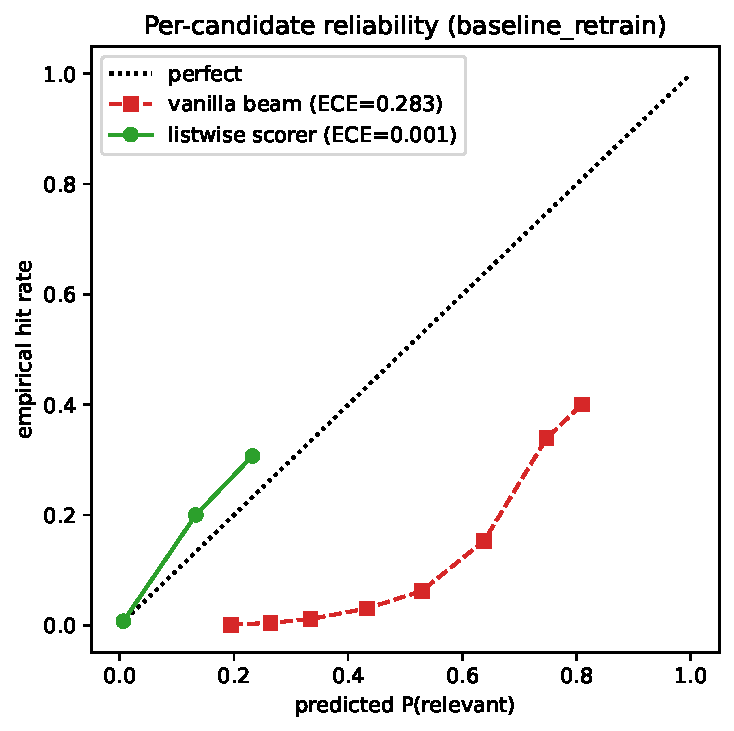
\includegraphics[width=0.8\linewidth]{figures/ece_reliability.pdf}
  \caption{Per-candidate reliability on MIND. The frozen generator's $\exp(\mathrm{avg\_logprob})$ is
  far above the diagonal (overconfident, ECE 0.283); the listwise scorer's probability tracks the
  diagonal (ECE 0.0009).}
  \label{fig:ece}
\end{figure}

\paragraph{Ablations.} (i) \emph{Loss $\times$ label} (MIND): over
$\{\text{bce},\text{listmle},\text{approxndcg}\}\times\{\text{binary},\text{soft}\}$, binary BCE is the
grid maximum (0.0381 $R@1$), justifying the locked choice. (ii) \emph{$\lambda$-sensitivity}
(Fig.~\ref{fig:lambda}): the chosen $\lambda^\star$ shrinks as Scoring Efficiency rises (MIND
$\lambda^\star{=}0.1$ at SE 9\%, Amazon $\lambda^\star{=}0.02$ at SE 12--19\%).

\begin{figure}[t]
  \centering
  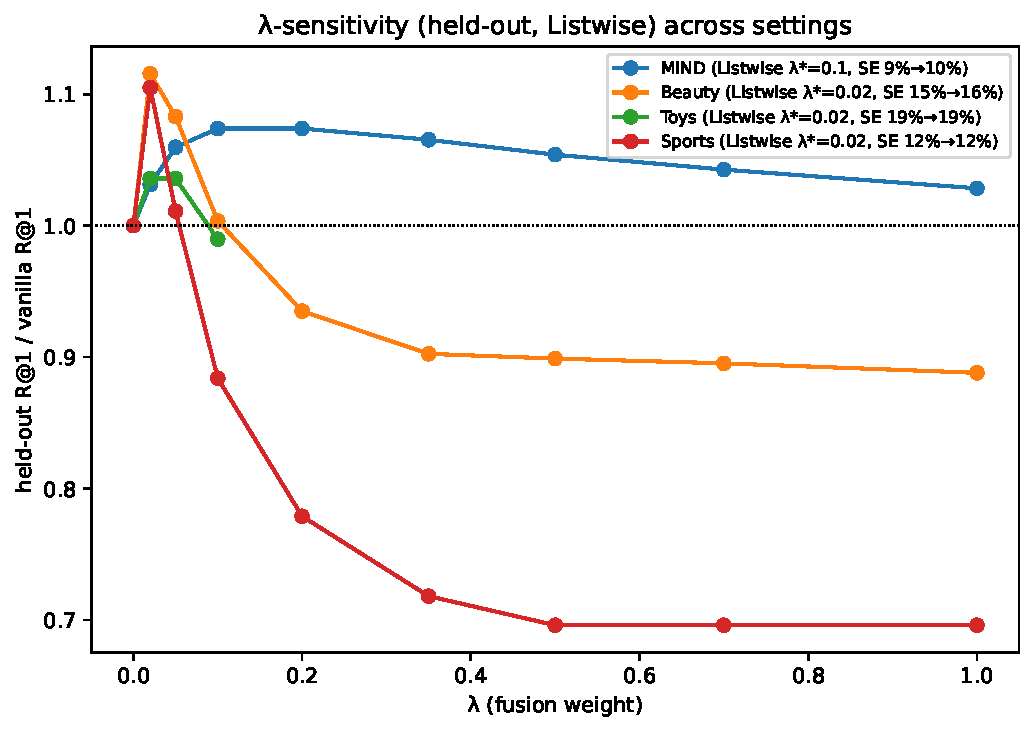
\includegraphics[width=\linewidth]{figures/lambda_sensitivity.pdf}
  \caption{$\lambda$-sensitivity (held-out, Listwise) across the four settings, normalized to vanilla
  ($\lambda{=}0$). Higher-Scoring-Efficiency settings prefer a smaller $\lambda^\star$.}
  \label{fig:lambda}
\end{figure}

\section{Limitations}
The generative rows are beam-recall-bounded; we do not claim absolute-metric superiority over
full-catalog discriminative models, only a controlled within-generator improvement (reported
honestly). Recall@1 significance is weak under leave-one-out (single relevant target); we rely on
Recall@10. $\lambda$ is not dimensionless across base models, so its absolute value is not
cross-setting comparable; we report $\lambda^\star\!\leftrightarrow\!$SE only as a trend. We evaluate
four settings and two base architectures; broader generality (large-scale, cross-lingual) is future
work.

\section{Conclusion}
A frozen generative retriever's overconfident beam scores leave a large, recoverable ranking gap. A
small post-hoc scorer with a held-out $\lambda$-selection closes it across diverse base
generators, domains, and code-lengths---a model-agnostic, retrain-free improvement.

\bibliographystyle{ACM-Reference-Format}
\bibliography{references}

\end{document}
